{
Denne udvidelse sigter mod at forbedre den eksisterende bedømmelse af
interessante regioner i forhold til det gyldne snit. Specielt er der
en type af interessante regioner som bliver fravalgt af den naive
metode, nemlig regioner med massemidtpunkt i det gyldne snit, men med et
afgrænsende rektangel uden for margin. Et eksempel på dette kan ses i
figur \ref{hus}, hvor den sorte region ikke anses som liggende i det
gyldne snit af den naive fremgangsmåde. Vi vil gerne have at sådanne
regioner klassificeres som en positiv interessant region.

\begin{figure}[h]
	\begin{center}
		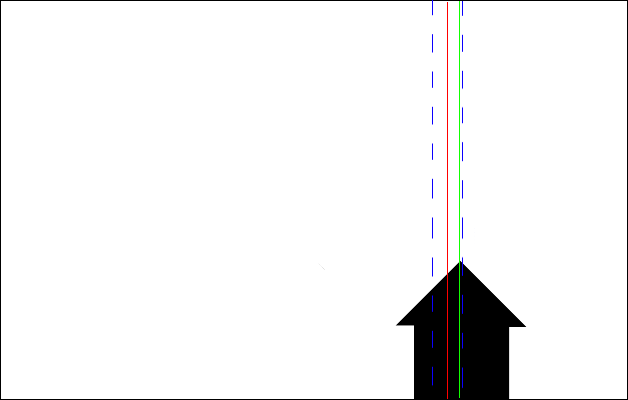
\includegraphics[scale=0.3,angle=0]{afsnit/vores_implementation/billeder/udvidet_loesning/husworks.png}
	\end{center}
	\caption[]{Et hus som bliver skåret over så midten ligger inde for snittet margin}
	\label{hus}
\end{figure}


\subsubsection{Opdeling af region med et grid}
% Original
%\subsubsection{Opdeling af ragion med et grid}
Måden vi deller ragionen op på, er hved hjælp af et gridt som vi
tilføjer vær baunding box, se figur \ref{grid}. Da vi ved hvilken farve
baunding boxens ragion er, tager vi alle de punkter i grittet som har
denne farve, og få der ved en bedre beskrivels af hvordan ragionen ser
ud. For at gøre algoritmen lidt hurtiger, er vores gridt punkter lavet
med 1 pixels mellemrum.

\begin{figure}[h]
	\centering
	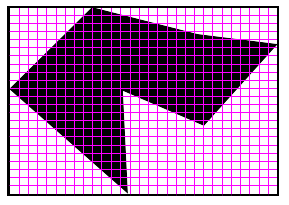
\includegraphics[scale=0.76,angle=0]{afsnit/vores_implementation/billeder/udvidet_loesning/udvidetloesninglayer.png}
	\caption[]{Et grid over en ragion i baunding box}
	\label{grid}
\end{figure}

\subsubsection{Bedømmelse med hensyn til massemidtpunkt}
Givet en region $R$ betegner vi antallet af punkter i regionen med
$|R|$. Vi antager at vi betragter et vertikalt snit $G$ i et billede.
Det gælder for alle punkter $p \in R$ at de kan befinde sig ovenpå, til
højre eller til venstre for $G$. I denne sammenhæng lader vi $R_r$ og
$R_l$ beskrive punkter henholdsvis til højre og venstre for snittet $G$.
Afstanden fra en punkt til kanten af et billede kaldes $D_p$, hvor
kanten er origo i billedet. Med disse informationer kan vi afgøre om
snitte deler regionen to lige store dele, samt om store dele af regionen
befinder sig langt væk fra snittet. Vi vil gerne kigge på en regions
massemidtpunkt og se om dette ligger inden for margin. Vi beregner
regionens massemidtpunkt ved funktionen


\begin{eqnarray}
    m(R) & = & \frac{\sum_{p \in R}{D_p}}{|R|} \label{masssemidpunkt}
    \label{MPunkt}
\end{eqnarray}

hvor m(R) giver os en værdi for hvad for et lige linie der delle ragionen
op i 2 delle, som er mest ens.

\begin{figure}[h]
	\begin{center}
		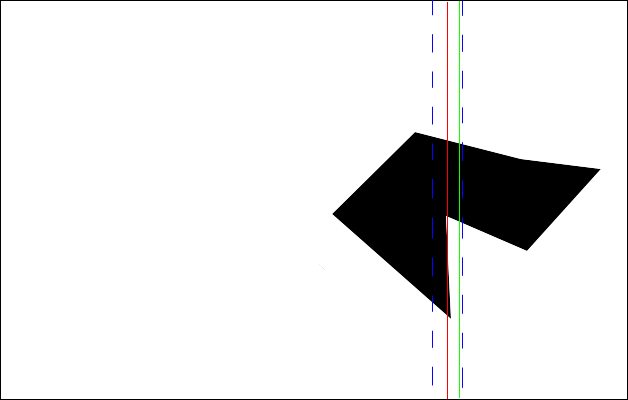
\includegraphics[scale=0.5,angle=0]{afsnit/vores_implementation/billeder/udvidet_loesning/cOMCutMargin.png}
	\end{center}
	\caption[]{Regioner hvor massemidtpunktet, snit og margin er tegnet ind, som man kan se ligger midtpunktet inde for marginen}
	\label{cOMCutMargin}
\end{figure}

Hvis $m(R)$ ligger inden for margin, se figur \ref{cOMCutMargin}. Bliver
regionen godtaget som liggende i snittet. Det er dog ikke helt nok kun
at bedømme regionerne efter massemidtpunkt, da man kan konstruere en
region som vi ikke vil godtage, men som har massemidtpunkt inde for
marginen, se figur \ref{dontwork}. 

\begin{figure}[h]
	\begin{center}
		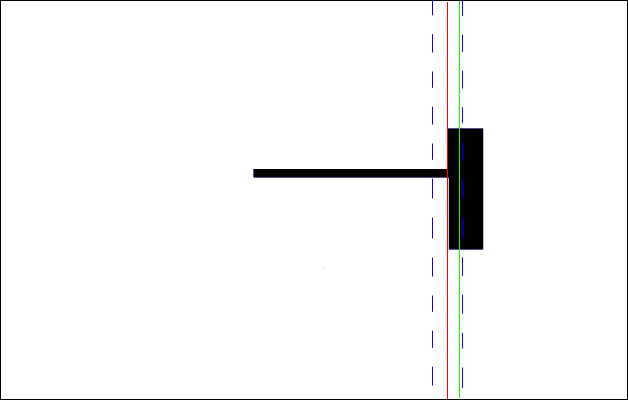
\includegraphics[scale=0.5,angle=0]{afsnit/vores_implementation/billeder/udvidet_loesning/dontWork.png}
	\end{center}
	\caption[]{Figur som har et massemidtpunkt indenfor margin, men vi ikke vil have med i godtaget regioner, på grund af den lange stang}
	\label{dontwork}
\end{figure}

Måden vi få løst problemet på er ved at lave en nyt tjek som kan sortere
de regioner fra som vi ikke vil have godkende. Det gør vi hjælp af
funktion

\begin{eqnarray}
    f(R) & = & \frac{|R_{l}| - |R_{r}|}{|R|}
    \label{Fordeling}
\end{eqnarray}

Som sammenligner antal pixels på begge sider af snittet og giver en
procent på hvor stor forskel der er, det vil sige at $f(R) \in [-1,1]$.
Hvis $f(R)$ er positivt, er der $f(R)$ procent flere pixels på $|R_l|$
side og vise verser. hvis den abselutte værdig af $f(R)$ er over $0.75$
betyder det at regionen er få skævt fordelt og den sortere den fra. Få
at give et eksempel på hvornår vores naive algoritme virker, se figur \ref{centerOfMass}
\begin{figure}[h]
	\begin{center}
		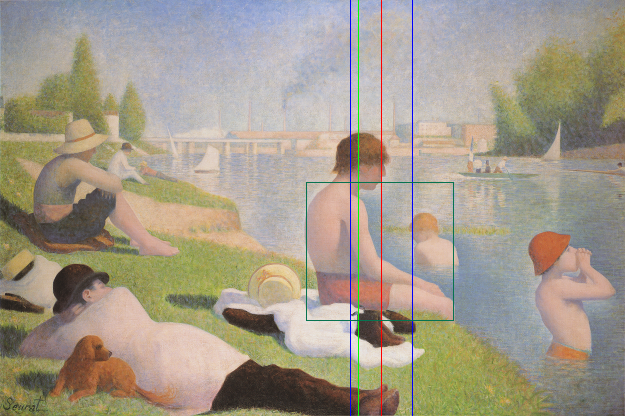
\includegraphics[scale=0.35,angle=0]{afsnit/vores_implementation/billeder/udvidet_loesning/centerOfMass.png}
	\end{center}
	\caption[]{Eksempel på hvordan den udvidet algoritme virker på et billedet hvor den naive algoritme ikke vil have fundet det}
	\label{centerOfMass}
\end{figure}

\clearpage

}

% vim: set tw=72 spell spelllang=da:
